\section*{Additional Figures}

\subsection*{Language Speed}

\begin{figure}[H]
	\centering
	\includegraphics[width=0.8\textwidth]{figures/thread_performance.png}
	\caption{Comparison of a minimal test program to compare best case thread sample rates in C and Python; each point is an average over 50000 samples. Note that both trends are linear, but a logarithmic scale had to be used to compare the datasets on the same graph.}
	\label{thread_performance.png}
\end{figure}


\begin{figure}[H]
	\centering
	\includegraphics[width=0.8\textwidth]{figures/thread_deviation.png}
	\caption{The standard deviations of the distributions in Figure \ref{thread_performance.png}. It should be noted that the distributions are not gaussian.}
\end{figure}




\subsection*{Data storage Efficiency}

\begin{figure}[H]
	\centering
	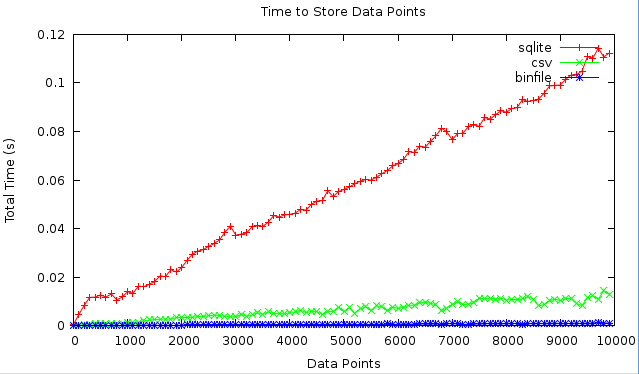
\includegraphics[width=0.8\textwidth]{figures/data_storespeed.png}
	\caption{Efficiency of different data storage methods. Although a data base provides many advanced features, it was realised that these features were not really needed for storing time ordered sensor data.}
\end{figure}

\subsection*{Sampling Rates}

\begin{figure}[H]
	\centering
	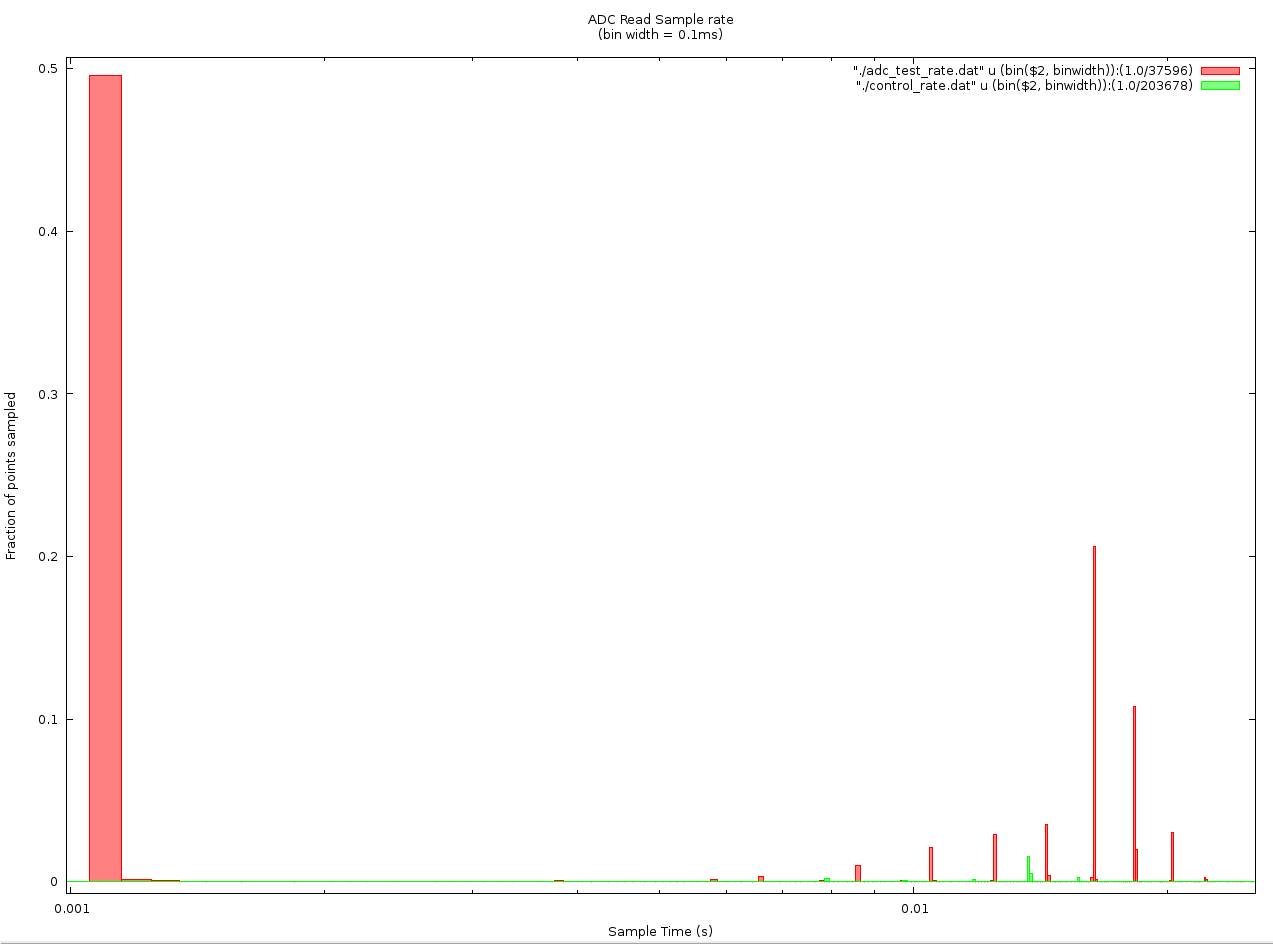
\includegraphics[width=0.8\textwidth]{figures/adc_histogram.png}
	\caption{Same graph as Figure \ref{sample_rate_histogram.png} but zoomed in to highlight the distribution obtained with \funct{ADC_Read} is called.}
\end{figure}


\begin{figure}[H]
	\centering
	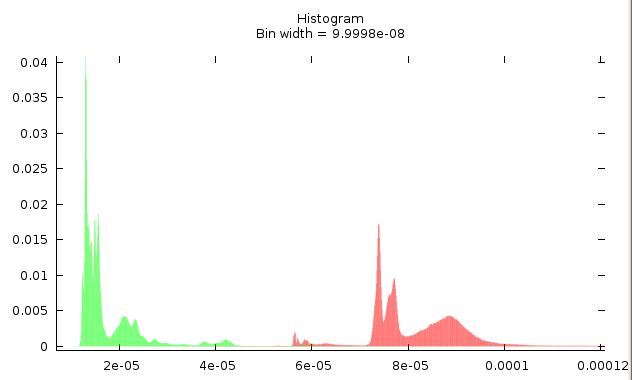
\includegraphics[width=0.8\textwidth]{figures/rt_vs_normal_3-2-0-4-amd64_1e-6s.png}
	\caption{Distributions (nanosecond timestamp resolution) for Real Time Linux kernel (\textcolor{green}{green}) and ``Vanilla'' Linux kernel (\textcolor{red}{red}) running on an i5 laptop with the sample rate set to 1$\mu\text{s}$}
\end{figure}


\begin{figure}[H]
	\centering
	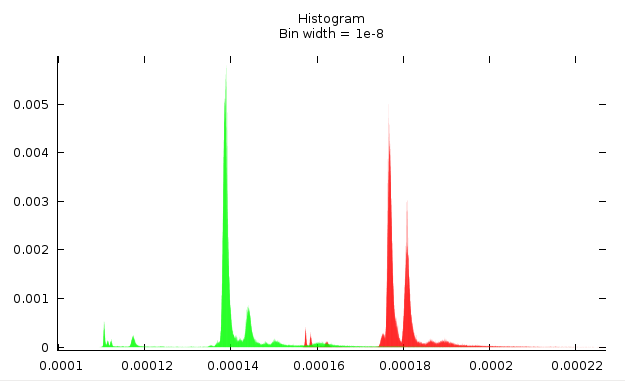
\includegraphics[width=0.8\textwidth]{figures/rt_vs_normal_3-2-0-4-amd64_1e-4s.png}
	\caption{As above but with a 100$\mu\text{s}$ sample rate}
\end{figure}


